\documentclass[10pt]{article}
\usepackage[a4paper]{geometry}
\usepackage{amsmath}
\usepackage{amssymb}
\usepackage{tocbibind}
\usepackage{graphicx}
\usepackage{hyperref}
\usepackage{mdframed}
\usepackage{subfiles}
\usepackage{titlesec}
\usepackage[dvipsnames]{xcolor}

%%%%%%%%%%%%%%%%%%%%%%%%%%%%%%%%%%%%%%%%%%%%%%%%%%%%%%%%%%%%%%%%%%%%%%%% Setups
\newcommand{\Eq}[1]{Equation~\ref{eq:#1}}
\newcommand{\Fig}[1]{Figure~\ref{fig:#1}}

\newenvironment{textbox}[1]
{%
  \mdfsetup{%
    frametitle={\colorbox{white}{\space#1\space}},
    frametitleaboveskip=-\ht\strutbox,
  }
  \begin{mdframed}
}
{
  \end{mdframed}
}

\setlength\parindent{0pt}
\graphicspath{{./fig/}}

\hypersetup{%
  hidelinks,
  colorlinks,
  citecolor={YellowOrange!85!black},
  linkcolor={Aquamarine!85!black},
  bookmarksopen=true,
  bookmarksnumbered=true,
  linktoc=all,
  pdfauthor=Jihang Li,
}

\title{Notes of ``Human-centric Indoor Scene Synthesis Using Stochastic Grammar''}
\author{Jihang Li}
%%%%%%%%%%%%%%%%%%%%%%%%%%%%%%%%%%%%%%%%%%%%%%%%%%%%%%%%%%%%%%%%%%%%%%%%%%%%%%%

\begin{document}
\maketitle
\tableofcontents

%%%%%%%%%%%%%%%%%%%%%%%%%%%%%%%%%%%%%%%%%%%%%%%%%%%%%%%%%%%%%%%%%%%%%% Abstract
\section*{Abstract}%
\label{sec:abstract}
 Human contexts as contextual relations are encoded by \textbf{Markov Random
 Field (MRF)} on the terminal nodes.

 Distributions are learned from an indoor scene dataset.

 New layers are sampled using \textbf{Monte Carlo Markov Chain (MCMC)}.

 Sampling is based on three criteria:
 %
\begin{enumerate}
  \item Visual realism compare to SOTA room arrangement method.
  \item Accuracy of the affordance maps w.r.t.\ ground-truth.
  \item The functionality and naturalness of synthesized rooms evaluated by
    human subjects.
\end{enumerate}

%%%%%%%%%%%%%%%%%%%%%%%%%%%%%%%%%%%%%%%%%%%%%%%%%%%%%%%%%%%%%%%%%%%%% Chapter 1
\section{Introduction}%
\label{sec:introduction}
Traditional methods of image data collection and labeling limitations:
%
\begin{enumerate}
  \item High-quality ground truths are hard to obtain, as depth and surface
    normal obtained from sensors are always noisy.
  \item Impossible to label certain ground truth information.
  \item Manual labeling of massive ground-truth is tedious and error-prone.
\end{enumerate}

The proposed algorithm is useful for (but not limited to):
%
\begin{enumerate}
  \item Learning and inference for computer vision tasks.
  \item 3D content generation.
  \item 3D reconstruction and robot mappings.
  \item Benchmarking of both low-level and high-level task-planning problems in
    robotics.
\end{enumerate}

Four major difficulties in synthesizing:
%
\begin{enumerate}
  \item The number of pieces may vary in a functional group. (e.g.\ a dinning
    set.)
  \item There is already a quadratic number of object-object relation even if
    only pair-wise relations are considered.
  \item Most object-object relations are not obviously meaningful. (e.g.\ a pen
    and a monitor both on a desk.)
  \item An excessive number of constrains are generated due to the previous
    difficulties.
\end{enumerate}

Contributions:
%
\begin{enumerate}
  \item Jointly model objects, affordances, and activity planning for indoor
    scene configurations.
  \item Provide a general learning and sampling framework for indoor scene
    modeling.
  \item Demonstrate the effectiveness of this structured joint sampling by
    extensive comparative experiments.
\end{enumerate}


%%%%%%%%%%%%%%%%%%%%%%%%%%%%%%%%%%%%%%%%%%%%%%%%%%%%%%%%%%%%%%%%%%%%% Chapter 2
\section{Representation of Indoor Scenes}%
\label{sec:representation}
An attributed S-AOG combines:
%
\begin{enumerate}
  \item A \textbf{probabilistic context free grammar (PCFG)}.
  \item Contextual relations defined on an MRF, i.e.\ the horizontal links
    among the nodes.
\end{enumerate}

An S-AOG is defined as a 5-tuple: $\mathcal{G} = \langle S, V, R, P, E \rangle$,
where:
%
\begin{itemize}
  \item $S$: the root node of the scene grammar
  \item $V$: the vertex set
    \begin{itemize}
      \item $V = V_{NT} \cup V_T$
      \item $V_{NT} = V^{And} \cup V^{Or} \cup V^{Set}$\footnote{$V^{Set}$: A
          set of Or-nodes serving as child branches are grouped by an And-node,
          and each child branch may include different numbers of objects.}
      \item $V_T = V^r_T \cup V^a_T$
        \begin{enumerate}
          \item Regular terminal node: $v \in V^r_T$, represents a spatial
            entity in a scene with \textbf{internal attributes} of object sizes
            $(w, l, h), and $\textbf{external attributes} $A_{ext}$ of
            object position $(x, y, z)$ and orientation ($x --- y$ plane)
            $\theta$ and sampled human positions.
          \item Address terminal node: $v \in V^a_T$, encodes interactions that
            only occur in a certain context but a absent in all others.
        \end{enumerate}
    \end{itemize}
  \item $R$: the production rules
  \item $P$: the probability model
  \item $E$: the contextual relations, $E = E_f \cup E_o \cup E_g \cup E_r$
    \begin{itemize}
      \item $E_f$: relations among furniture
      \item $E_o$: relations between supported objects and their supporting
        objects
      \item $E_g$: relations in a functional pair
      \item $E_r$: relations between furniture and the room
    \end{itemize}
\end{itemize}

\setcounter{figure}{2}
\begin{figure}[!htpb]
  \centering
  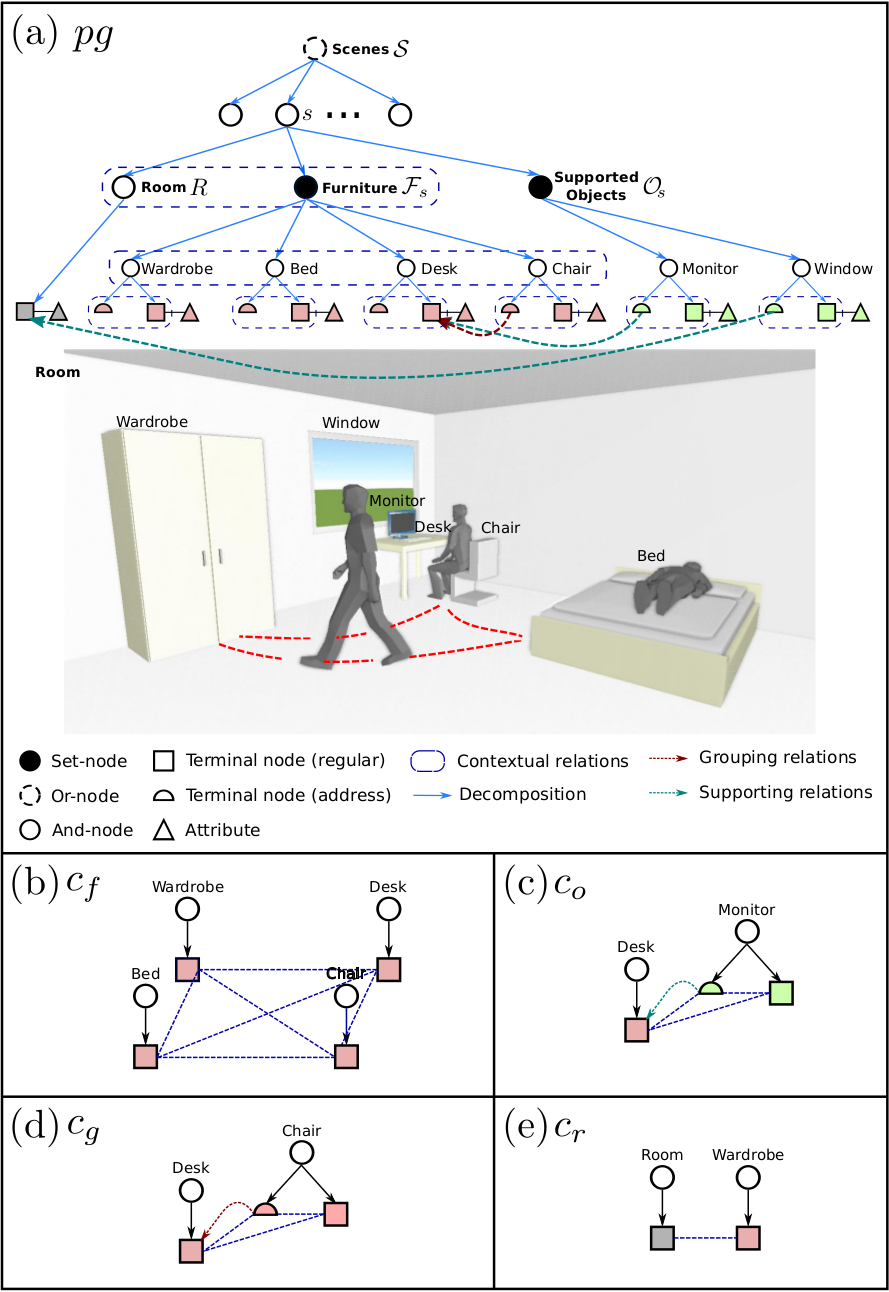
\includegraphics[width=0.6\linewidth]{fig_3.png}
  \caption{(a) A simplified example of a parse graph of a bedroom. The terminal
    nodes of the parse graph form an MRF in the terminal layer. Cliques are
    formed by the contextual relations projected to the terminal layer.
    Examples of the four types of cliques are shown in (b) --- (e),
    representing four different types of contextual relations.}%
  \label{fig:3}
\end{figure}


%%%%%%%%%%%%%%%%%%%%%%%%%%%%%%%%%%%%%%%%%%%%%%%%%%%%%%%%%%%%%%%%%%%%% Chapter 3
\section{Probabilistic Formulation of S-AOG}%
\label{sec:formulation}
The prior probability of $pg$ generated by an S-AOG parameterized by $Theta$ is
formulated as a \textbf{Gibbs distribution}:
%
\begin{align}
  p(pg \vert \Theta) &= \frac{1}{Z} \{-\mathcal{E}(pg \vert \Theta)\} \label{eq:1} \\
                     &= \frac{1}{Z} \{-\mathcal{E}(pt \vert \Theta) - \mathcal{E}(E_{pt} \vert \Theta)\}, \label{eq:2}
\end{align}
%
where:
%
\begin{itemize}
  \item $\mathcal{E}(pg \vert \Theta)$: the energy function of a $pg$
  \item $\mathcal{E}(pt \vert \Theta)$: the energy function of a $pt$
  \item $\mathcal{E}(E_{pt} \vert \Theta)$: the energy term of the contextual
    relations
\end{itemize}
%
$\mathcal{E}(pt \vert \Theta)$ can be decomposed into:
%
\begin{align}
  \label{eq:3}
  \mathcal{E}(pt \vert \Theta) = \underbrace{\sum_{v \in V^{Or}} \mathcal{E}^{Or}_{\Theta}(v) + \sum_{v \in V^{Set}} \mathcal{E}^{Set}_{\Theta}(v)}_{\text{non-terminal nodes}} + \underbrace{\sum_{v \in V^r_T} \mathcal{E}^{A_{in}}_{\Theta}(v)}_{\text{terminal nodes}},
\end{align}
%
where the choice of the child node an Or-node and the child branch of a
Set-node \textbf{follow different multinomial distributions}. $A_{in}$ of
terminal nodes \textbf{follows a non-parametric probability distribution
learned by kernel density estimation}.


%%%%%%%%%%%%%%%%%%%%%%%%%%%%%%%%%%%%%%%%%%%%%%%%%%%%%%%%%%%%%%%%%% Bibliography
% \bibliographystyle{plain}
% \bibliography{part_ii/part_ii}

\end{document}
